\chapter{Evaluation}
\label{chap:evaluation}

\section{Experimental Setup}
\label{sec:experimental_setup}

We evaluate the platform and the algorithm through a controlled factorial experiment that varies three system dimensions: \textbf{LLM providers} (commercial vs.\ open-source models), \textbf{prompting strategies} (direct vs.\ chain-of-thought), and \textbf{decision modes} (single-agent vs.\ ensemble). All experiments use the same dataset and target ontology and follow a breadth-first traversal rooted at \texttt{owl:Thing}; only the configuration variables defined below are varied.

% -----------------------------------------------------------------------------
% Subsection: Dataset
% -----------------------------------------------------------------------------
\subsection{Dataset}
\label{subsec:dataset}

\paragraph{Tables.}
The evaluation is conducted on a domain-specific benchmark comprises real-world tabular data collected from heterogeneous building management systems and energy audits. The benchmark consists of 47 distinct tables containing a total of 431 columns. Each column is treated as an independent semantic annotation instance. Domain experts assign each column a terminal BEO class; the corresponding \emph{root-to-leaf} ontology path serves as the \textit{gold standard} for both node-level and path-level evaluation.

\paragraph{Ontology.}
The experiments utilize the \textbf{Building Energy Ontology (BEO)} as the target concept space. This ontology comprises 602 classes organized into a hierarchy with a maximum depth of 8. The class hierarchy is formally represented as a Directed Acyclic Graph (DAG) derived principally from \texttt{rdfs:subClassOf} relations. All traversals originate from the universal root \texttt{owl:Thing}; no synthetic super-roots are introduced. During annotation, candidate classes at depth $d$ are generated strictly by expanding the children of the current frontier nodes. Figure~\ref{fig:ontology_example} illustrates a representative fragment of the BEO ontology structure.

% FIGURE: Ontology Example
\begin{figure}[htbp]
    \centering
    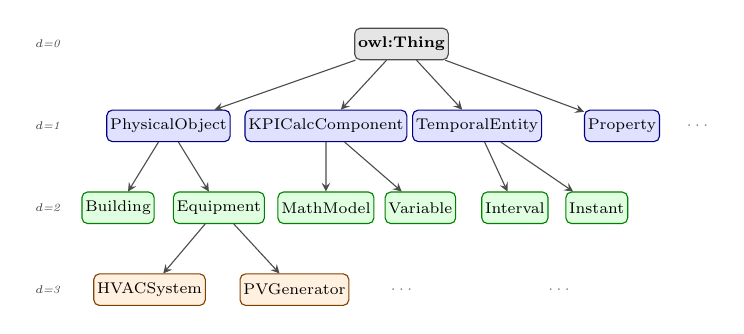
\begin{tikzpicture}[
    scale=0.8, transform shape,
    every node/.style={font=\scriptsize},
    class/.style={rectangle, rounded corners=2pt, draw, minimum height=5mm, align=center, inner sep=1.5pt},
    root/.style={class, fill=gray!20, draw=gray!60!black, font=\scriptsize\bfseries},
    level1/.style={class, fill=blue!12, draw=blue!50!black},
    level2/.style={class, fill=green!12, draw=green!50!black},
    level3/.style={class, fill=orange!12, draw=orange!50!black},
    edge/.style={draw, ->, >=stealth, gray!60!black},
    depthlabel/.style={font=\tiny\itshape, text=gray!50!black}
]

% Depth labels on the left (moved further left)
\node[depthlabel, anchor=east] at (-0.8, 0) {$d$=0};
\node[depthlabel, anchor=east] at (-0.8, -1.3) {$d$=1};
\node[depthlabel, anchor=east] at (-0.8, -2.6) {$d$=2};
\node[depthlabel, anchor=east] at (-0.8, -3.9) {$d$=3};

% Level 0: Root
\node[root] (thing) at (4.5, 0) {owl:Thing};

% Level 1: Top-level categories (from BEO ontology)
\node[level1] (physical) at (0.8, -1.3) {PhysicalObject};
\node[level1] (kpicomp) at (3.3, -1.3) {KPICalcComponent};
\node[level1] (temporal) at (5.7, -1.3) {TemporalEntity};
\node[level1] (property) at (8, -1.3) {Property};

% Level 2: Sub-categories
\node[level2] (building) at (0, -2.6) {Building};
\node[level2] (equipment) at (1.6, -2.6) {Equipment};
\node[level2] (mathmodel) at (3.3, -2.6) {MathModel};
\node[level2] (variable) at (4.8, -2.6) {Variable};
\node[level2] (interval) at (6.3, -2.6) {Interval};
\node[level2] (instant) at (7.6, -2.6) {Instant};

% Level 3: Leaf classes (moved apart to avoid overlap)
\node[level3] (hvac) at (0.5, -3.9) {HVACSystem};
\node[level3] (pv) at (2.8, -3.9) {PVGenerator};

% Edges from root
\draw[edge] (thing) -- (physical);
\draw[edge] (thing) -- (kpicomp);
\draw[edge] (thing) -- (temporal);
\draw[edge] (thing) -- (property);

% Edges from Level 1
\draw[edge] (physical) -- (building);
\draw[edge] (physical) -- (equipment);
\draw[edge] (kpicomp) -- (mathmodel);
\draw[edge] (kpicomp) -- (variable);
\draw[edge] (temporal) -- (interval);
\draw[edge] (temporal) -- (instant);

% Edges from Level 2
\draw[edge] (equipment) -- (hvac);
\draw[edge] (equipment) -- (pv);

% Ellipsis nodes to indicate more classes
\node[font=\scriptsize, text=gray] at (4.5, -3.9) {$\cdots$};
\node[font=\scriptsize, text=gray] at (7, -3.9) {$\cdots$};
\node[font=\scriptsize, text=gray] at (9.2, -1.3) {$\cdots$};

\end{tikzpicture}

    \caption[BEO ontology structure]{A fragment of the BEO ontology hierarchy. The ontology is organized as a DAG rooted at \texttt{owl:Thing}, with domain-specific classes such as \texttt{Equipment}, \texttt{Measurement}, and \texttt{TemporalEntity} at intermediate levels.}
    \label{fig:ontology_example}
\end{figure}

% -----------------------------------------------------------------------------
% Subsection: Preprocessing
% -----------------------------------------------------------------------------
\subsection{Preprocessing}
\label{subsec:eval_preprocessing}

To isolate the behaviour of the annotation logic, the system encodes each column using a uniform context representation comprising three elements: the original column header string, a coarse inferred type hint (e.g., Numeric, String), and a set of representative sample values selected using a \textit{Head-K} policy with $k=5$. These features form the only table-derived input to the LLM-based decision modules. No table-level descriptions or external knowledge-base signals are injected, so the evaluation reflects reasoning from column-local evidence alone.

% -----------------------------------------------------------------------------
% Subsection: Evaluation Metrics
% -----------------------------------------------------------------------------
\subsection{Evaluation Metrics}
\label{sec:eval_metrics}

We evaluate annotation quality at two granularities using set-based precision, recall, and F$_1$ metrics at node level and path level. Let $\mathcal{D} = \{(x_i, Y_i, \hat{Y}_i)\}_{i=1}^{N}$ denote the evaluation set, where $x_i$ is a column, $Y_i$ is the set of ground-truth ontology paths, and $\hat{Y}_i$ is the set of predicted paths. Each path is a sequence of class labels from root to leaf (e.g., $\langle\texttt{Thing}, \texttt{Measurement}, \texttt{Currency}\rangle$).

\paragraph{Node-Level Metrics.}
Node-level evaluation assesses the coverage of individual ontology classes along the predicted paths. We define a flattening operator $\mathcal{N}(\cdot)$ that extracts all unique class labels from a set of paths:
\begin{equation}
    \mathcal{N}(Y) = \bigcup_{p \in Y} \{c : c \in p\}
\end{equation}
For each instance $i$, we compute confusion counts over the flattened class sets:
\begin{align}
    \text{TP}_i &= |\mathcal{N}(\hat{Y}_i) \cap \mathcal{N}(Y_i)|, \quad
    \text{FP}_i = |\mathcal{N}(\hat{Y}_i) \setminus \mathcal{N}(Y_i)|, \quad
    \text{FN}_i = |\mathcal{N}(Y_i) \setminus \mathcal{N}(\hat{Y}_i)|
\end{align}

\paragraph{Path-Level Metrics.}
Path-level evaluation applies \textbf{strict path equality}: a prediction is correct only if the entire class sequence matches the ground truth exactly. Two paths $p$ and $q$ are equal iff $|p| = |q|$ and $p_j = q_j$ for all $j \in \{1, \ldots, |p|\}$. Confusion counts are computed directly on path sets:
\begin{align}
    \text{TP}_i &= |\hat{Y}_i \cap Y_i|, \quad
    \text{FP}_i = |\hat{Y}_i \setminus Y_i|, \quad
    \text{FN}_i = |Y_i \setminus \hat{Y}_i|
\end{align}
Under this strict criterion, a single incorrect branch decision at any traversal depth invalidates the entire path.

\paragraph{Aggregation: Micro- vs.\ Macro-Averaging.}

We report both micro- and macro-averaged metrics to characterize performance under class imbalance. 

\textbf{Micro-averaging} aggregates confusion counts across all instances before computing metrics, thereby weighting each prediction equally:
\begin{equation}
    P_{\mu} = \frac{\sum_{i=1}^{N} \text{TP}_i}{\sum_{i=1}^{N} (\text{TP}_i + \text{FP}_i)}, \quad
    R_{\mu} = \frac{\sum_{i=1}^{N} \text{TP}_i}{\sum_{i=1}^{N} (\text{TP}_i + \text{FN}_i)}, \quad
    F_{1,\mu} = \frac{2 P_{\mu} R_{\mu}}{P_{\mu} + R_{\mu}}
\end{equation}

\textbf{Macro-averaging} computes per-instance metrics and averages uniformly, giving equal weight to each column regardless of path cardinality:
\begin{equation}
    P_i = \frac{\text{TP}_i}{\text{TP}_i + \text{FP}_i}, \quad
    R_i = \frac{\text{TP}_i}{\text{TP}_i + \text{FN}_i}, \quad
    F_{1,i} = \frac{2 P_i R_i}{P_i + R_i}
\end{equation}
\begin{equation}
    P_M = \frac{1}{N}\sum_{i=1}^{N} P_i, \quad
    R_M = \frac{1}{N}\sum_{i=1}^{N} R_i, \quad
    F_{1,M} = \frac{1}{N}\sum_{i=1}^{N} F_{1,i}
\end{equation}

The BEO benchmark exhibits a long-tailed class distribution: a small number of frequent classes account for a disproportionate share of annotations, while many classes appear rarely. Micro-averaging tends to reflect performance on frequent classes, whereas macro-averaging penalizes errors on minority classes more heavily. We report both to provide a complete picture: micro-F$_1$ indicates aggregate predictive utility, while macro-F$_1$ reveals robustness across the class distribution. 

We additionally report total time as a deployment-relevant indicator of end-to-end efficiency.

% -----------------------------------------------------------------------------
% Subsection: Experiment Matrix
% -----------------------------------------------------------------------------
\subsection{Experiment Matrix}
\label{subsec:experiment_matrix}

We evaluate 8 distinct configurations defined by the Cartesian product of three variables:
\begin{equation}
    \text{Config} \in \text{Provider} \times \text{Prompt} \times \text{Decision Mode}
\end{equation}
where:
\begin{itemize}
    \item $\text{Provider} \in \{ \texttt{Azure (GPT-4.1)}, \texttt{Ollama (GPT-OSS:20b)} \}$
    \item $\text{Prompt} \in \{ \texttt{Direct}, \texttt{CoT} \}$
    \item $\text{Decision Mode} \in \{ \texttt{Single}, \texttt{EDM} \}$
\end{itemize}

\paragraph{Prompting Styles.}
\textbf{Direct} prompting instructs the model to return a classification decision without explicit intermediate reasoning. \textbf{Chain-of-Thought (CoT)} prompting requires the model to produce a brief reasoning trace before outputting the final decision.

\paragraph{Decision Modes.}
Under \textbf{Single} mode, decisions are rendered by a single LLM judgment per candidate set. Under \textbf{EDM} mode, decisions are produced via multi-agent voting with fixed hyperparameters: $\beta=30$ (classes per agent), $\alpha=3$ (agents per class), and $\theta=0.8$ (consensus threshold).

\paragraph{Execution Protocol.}
To minimize uncontrolled variance, all runs utilize a fixed temperature setting kept constant across providers and prompt styles. The pipeline operates sequentially: within a run, columns and EDM agent calls are executed with an effective parallelism of 1. Consequently, the reported total time represents wall-clock runtime per experiment run, encompassing API latency and orchestration overhead. Table~\ref{tab:experiment_matrix} summarizes all eight configurations.

% TABLE: Experiment Matrix
\begin{table}[htbp]
    \centering
    \caption{Experiment configuration matrix.}
    \label{tab:experiment_matrix}
    \renewcommand{\arraystretch}{1.2}
    \small
    \begin{tabular}{lcccc}
        \toprule
        \textbf{Run Name} & \textbf{Provider} & \textbf{Prompt} & \textbf{Mode} & \makecell{\textbf{EDM Params} \\ ($\beta/\alpha/\theta$)} \\
        \midrule
        \texttt{azure\_direct\_single} & Azure (GPT-4.1) & Direct & Single & -- \\
        \texttt{azure\_direct\_edm} & Azure (GPT-4.1) & Direct & EDM & 30/3/0.8 \\
        \texttt{azure\_cot\_single} & Azure (GPT-4.1) & CoT & Single & -- \\
        \texttt{azure\_cot\_edm} & Azure (GPT-4.1) & CoT & EDM & 30/3/0.8 \\
        \texttt{ollama\_direct\_single} & Ollama (GPT-OSS:20b) & Direct & Single & -- \\
        \texttt{ollama\_direct\_edm} & Ollama (GPT-OSS:20b) & Direct & EDM & 30/3/0.8 \\
        \texttt{ollama\_cot\_single} & Ollama (GPT-OSS:20b) & CoT & Single & -- \\
        \texttt{ollama\_cot\_edm} & Ollama (GPT-OSS:20b) & CoT & EDM & 30/3/0.8 \\
        \bottomrule
    \end{tabular}
\end{table}

% =============================================================================
% Section: Main Results
% =============================================================================
\section{Main Results}
\label{sec:main_results}

Table~\ref{tab:main_results} summarises the quantitative performance of the eight configurations defined in Section~\ref{sec:experimental_setup}. We report micro- and macro-averaged node- and path-level F$_1$ together with end-to-end wall-clock runtime. Under strict path equality, a single mistake at any depth invalidates the entire prediction, which systematically lowers path-level scores relative to node-level scores; the following subsections analyse the drivers of this gap.

% TABLE: Main Results
\begin{table}[htbp]
    \centering
    \caption{Main experimental results across 8 configurations. Node and path metrics are reported as F$_1$ scores (\%). Runtime is reported in seconds and minutes.}
    \label{tab:main_results}
    \renewcommand{\arraystretch}{1.2}
    \setlength{\tabcolsep}{4pt}
    \small
    \begin{tabular}{lcccccc}
        \toprule
        \multirow{2}{*}{\textbf{Configuration}} & \multicolumn{2}{c}{\textbf{Node F$_1$ (\%)}} & \multicolumn{2}{c}{\textbf{Path F$_1$ (\%)}} & \multicolumn{2}{c}{\textbf{Runtime}} \\
        \cmidrule(lr){2-3} \cmidrule(lr){4-5} \cmidrule(lr){6-7}
         & \textbf{Micro} & \textbf{Macro} & \textbf{Micro} & \textbf{Macro} & \textbf{(s)} & \textbf{(min)} \\
        \midrule
        \texttt{azure\_direct\_single} & 42.75 & 38.85 & 31.81 & 30.32 & 374 & 6.2 \\
        \texttt{azure\_direct\_edm}    & 46.23 & 37.27 & 33.54 & 29.45 & 2296 & 38.3 \\
        \texttt{azure\_cot\_single}    & \textbf{48.46} & \textbf{41.45} & \textbf{38.16} & \textbf{34.84} & 1434 & 23.9 \\
        \texttt{azure\_cot\_edm}       & 49.15 & 40.01 & 35.79 & 32.21 & 9088 & 151.5 \\
        \midrule
        \texttt{ollama\_direct\_single}  & 39.51 & 33.80 & 32.22 & 28.38 & 3789 & 63.1 \\
        \texttt{ollama\_direct\_edm}     & 39.30 & 29.96 & 27.03 & 23.82 & 34970 & 582.8 \\
        \texttt{ollama\_cot\_single}     & 36.39 & 30.71 & 28.67 & 25.14 & 8591 & 143.2 \\
        \texttt{ollama\_cot\_edm}        & 38.75 & 29.63 & 27.44 & 23.51 & 34916 & 581.9 \\
        \bottomrule
    \end{tabular}
\end{table}

% FIGURE: Results Comparison
\begin{figure}[htbp]
    \centering
    \includegraphics[width=\textwidth]{graphics/figures/results_comparison.pdf}
    \caption[Main results comparison]{Comparison of path and node F$_1$ (micro) across all 8 configurations. Azure (GPT-4.1) consistently outperforms Ollama (GPT-OSS:20b).}
    \label{fig:results_comparison}
\end{figure}

% -----------------------------------------------------------------------------
% Subsection: Overall Comparison
% -----------------------------------------------------------------------------
\subsection{Overall Comparison}
\label{subsec:results_overall}

Two high-level trends emerge from Table~\ref{tab:main_results}:

\begin{enumerate}
    \item \textbf{Best path-level performance.} The strongest path-level scores are achieved by \texttt{azure\_cot\_single} (path F$_1$ micro: 38.16\%, macro: 34.84\%), indicating that explicit reasoning improves hierarchical disambiguation under column-local context.
    \item \textbf{Large runtime dispersion.} End-to-end runtime spans orders of magnitude: \texttt{azure\_direct\_single} completes in 6.2 minutes, whereas \texttt{ollama\_*\_edm} exceeds 9.6 hours. Under sequential execution, inference cost scales with the number of LLM calls per column and dominates overall latency.
\end{enumerate}

Micro-averaged scores generally exceed macro-averaged scores, consistent with a long-tailed class distribution in which macro averaging penalises errors on minority classes more strongly.

% -----------------------------------------------------------------------------
% Subsection: Effect of CoT Prompting
% -----------------------------------------------------------------------------
\subsection{Effect of Chain-of-Thought (CoT) Prompting}
\label{subsec:results_cot}

To isolate the impact of the prompting strategy, we compare Direct and CoT variants while keeping provider and decision mode fixed.

\paragraph{Azure (GPT-4.1).} CoT yields consistent accuracy gains:
\begin{itemize}
    \item \textbf{Single mode:} Path F$_1$ (micro) increases from 31.81\% to 38.16\% (+6.35pp), while runtime rises from 6.2 to 23.9 minutes.
    \item \textbf{EDM mode:} Path F$_1$ (micro) increases from 33.54\% to 35.79\% (+2.25pp), while runtime rises from 38.3 to 151.5 minutes.
\end{itemize}
For the high-capacity cloud model, CoT better integrates weak signals (header, type hint, sample values) and improves branch selection during traversal.

\paragraph{Ollama (GPT-OSS:20b).} In contrast, CoT does not provide a comparable benefit for the smaller local model:
\begin{itemize}
    \item \textbf{Single mode:} Path F$_1$ (micro) decreases from 32.22\% to 28.67\% (-3.55pp), while runtime increases from 63.1 to 143.2 minutes.
    \item \textbf{EDM mode:} CoT produces only marginal differences (27.03\% vs.\ 27.44\%).
\end{itemize}
These results suggest that the smaller model is more sensitive to longer prompts and the additional generation required by CoT. The extra reasoning text increases latency without consistently improving decision quality.

% FIGURE: CoT Effect
\begin{figure}[htbp]
    \centering
    \includegraphics[width=\textwidth]{graphics/figures/cot_effect.pdf}
    \caption[Effect of Chain-of-Thought prompting]{Effect of Chain-of-Thought (CoT) prompting on path-level F$_1$. CoT provides substantial gains for Azure (GPT-4.1) but offers minimal or negative improvement for Ollama (GPT-OSS:20b).}
    \label{fig:cot_effect}
\end{figure}

% -----------------------------------------------------------------------------
% Subsection: Effect of EDM
% -----------------------------------------------------------------------------
\subsection{Effect of Ensemble Decision Making (EDM)}
\label{subsec:results_edm}

EDM targets variance reduction by enforcing consensus ($\alpha=3$, $\theta=0.8$). The results indicate that strict voting introduces non-trivial accuracy--latency trade-offs under sequential execution.

\paragraph{Azure (GPT-4.1).} EDM is not uniformly beneficial:
\begin{itemize}
    \item Under Direct prompting, EDM improves path F$_1$ (micro) from 31.81\% to 33.54\%, but runtime increases by roughly a factor of six.
    \item Under CoT prompting, EDM reduces path F$_1$ (micro) from 38.16\% to 35.79\% while substantially increasing runtime.
\end{itemize}
This pattern suggests that when CoT already stabilises predictions, an additional strict voting layer may become overly conservative, pruning correct branches when agents disagree.

\paragraph{Ollama (GPT-OSS:20b).} For the local model, EDM performs poorly in the current configuration. Under Direct prompting, path F$_1$ (micro) drops from 32.22\% to 27.03\%, and runtime approaches ten hours. Given the sequential execution model, EDM multiplies the inference burden and is not practical at this scale without parallelisation.

% FIGURE: EDM Effect
\begin{figure}[htbp]
    \centering
    \includegraphics[width=\textwidth]{graphics/figures/edm_effect.pdf}
    \caption[Effect of Ensemble Decision Making]{Effect of Ensemble Decision Making (EDM) on path-level F$_1$. EDM provides modest gains under Direct prompting but can reduce accuracy when combined with CoT.}
    \label{fig:edm_effect}
\end{figure}


\paragraph{Level 1 Accuracy Analysis.} Since EDM targets variance reduction at each traversal step, we examine its effect specifically at the first hierarchy level (Level 1), where the candidate set is largest and decisions are most consequential for downstream accuracy. Table~\ref{tab:level1_accuracy} reports the proportion of columns for which at least one predicted Level 1 class matches the ground truth.

% TABLE: Level 1 Accuracy
\begin{table}[htbp]
    \centering
    \caption{Level 1 accuracy by configuration. Level 1 accuracy measures whether the predicted first-level class matches the ground truth.}
    \label{tab:level1_accuracy}
    \renewcommand{\arraystretch}{1.2}
    \small
    \begin{tabular}{lcc}
        \toprule
        \textbf{Configuration} & \textbf{Level 1 Accuracy (\%)} & \textbf{$\Delta$ vs Single} \\
        \midrule
        \texttt{azure\_direct\_single} & 51.7 & -- \\
        \texttt{azure\_direct\_edm} & 48.5 & $-3.2$ \\
        \texttt{azure\_cot\_single} & 52.0 & -- \\
        \texttt{azure\_cot\_edm} & 51.5 & $-0.5$ \\
        \midrule
        \texttt{ollama\_direct\_single} & 41.8 & -- \\
        \texttt{ollama\_direct\_edm} & 39.7 & $-2.1$ \\
        \texttt{ollama\_cot\_single} & 38.5 & -- \\
        \texttt{ollama\_cot\_edm} & 39.2 & $+0.7$ \\
        \bottomrule
    \end{tabular}
\end{table}

% FIGURE: Level 1 Accuracy
\begin{figure}[htbp]
    \centering
    \includegraphics[width=\textwidth]{graphics/figures/level1_accuracy.pdf}
    \caption[Level 1 accuracy comparison]{Level 1 accuracy comparing Single and EDM modes. Contrary to expectations, EDM does not consistently improve first-level decisions.}
    \label{fig:level1_accuracy}
\end{figure}

Contrary to the hypothesis that ensemble voting would improve decisions at the most ambiguous traversal step, EDM does not consistently outperform Single mode at Level 1. For Azure (GPT-4.1), EDM slightly reduces Level 1 accuracy under both Direct ($-3.2$pp) and CoT ($-0.5$pp) prompting. This suggests that the strict consensus threshold ($\theta=0.8$) may be overly conservative: when agents disagree on a correct but less obvious branch, the consensus mechanism may fail to select it. The results indicate that EDM's modest gains in overall path F$_1$ (Table~\ref{tab:main_results}) stem primarily from stabilizing later traversal steps rather than improving the critical first-level decision.

% =============================================================================
% Section: Case Analysis
% =============================================================================
\section{Case Analysis}
\label{sec:case_analysis}

Quantitative scores provide an overall comparison across configurations but do not explain why particular columns succeed or fail. The following case studies illustrate: (i) cases in which Chain-of-Thought (CoT) prompting resolves ambiguity, (ii) cases in which Ensemble Decision Making (EDM) stabilises traversal decisions, and (iii) recurring failure modes under column-local context constraints.

% -----------------------------------------------------------------------------
% Subsection: CoT Resolves Semantic Ambiguity
% -----------------------------------------------------------------------------
\subsection{CoT Resolves Semantic Ambiguity}
\label{subsec:case_cot}

This case illustrates the impact of explicit reasoning on an ambiguous currency-related column.

\begin{center}
\fbox{\begin{minipage}{0.95\textwidth}
    \small
    \textbf{Column context:}
    \begin{itemize}
        \item \textbf{Name:} \texttt{Cost (net in PLN)}
        \item \textbf{Type:} Numeric (float)
        \item \textbf{Samples:} \texttt{[1250.00, 890.50, 2100.00, ...]}
    \end{itemize}

    \textbf{Ground truth:} \\
    \texttt{Thing $\to$ Measurement $\to$ Currency}

	    \textbf{Predictions:}
	    \begin{itemize}
        \item \textbf{\texttt{azure\_direct\_single}:} \\
	        \texttt{Thing $\to$ KPIValue} \\
	        \textit{(Defaults to a generic value class and misses the currency semantics)}

        \item \textbf{\texttt{azure\_cot\_single}:} \\
        \texttt{Thing $\to$ Measurement $\to$ Currency} \\
        \textit{(Correctly identifies the currency measurement path)}
    \end{itemize}
\end{minipage}}
\end{center}

The token \enquote{PLN} provides a currency cue that is not captured by type hints or by the magnitudes of sample values. Under the \textbf{Direct} prompt, the model selects a generic value concept; under \textbf{CoT}, the model links \enquote{PLN} to a currency unit and selects the correct branch. Consequently, explicit reasoning primarily mitigates early branching errors when column-local evidence is sparse.

% -----------------------------------------------------------------------------
% Subsection: EDM Stabilises Selection
% -----------------------------------------------------------------------------
\subsection{EDM Stabilises Selection}
\label{subsec:case_edm}

This case shows how ensemble voting can achieve consensus on temporal concepts.

\begin{center}
\fbox{\begin{minipage}{0.95\textwidth}
    \small
    \textbf{Column context:}
    \begin{itemize}
        \item \textbf{Name:} \texttt{Month}
        \item \textbf{Type:} String
        \item \textbf{Samples:} \texttt{[2017-01, 2017-02, 2017-03, ...]}
    \end{itemize}

	    \textbf{EDM Voting at Level 0 (Parent: Thing):}
	    \begin{itemize}
	        \item \texttt{TemporalEntity}: 3/3 agents (100\%) -- \textbf{SELECTED}
	        \item \texttt{Observation}: 2/3 agents (67\%)
	        \item \texttt{Event}: 1/3 agents (33\%)
	        \item \texttt{Schedule}: 1/3 agents (33\%)
	    \end{itemize}
\end{minipage}}
\end{center}

EDM is beneficial when multiple plausible candidates exist at the same depth. Although individual agents proposed alternatives such as \texttt{Observation} or \texttt{Event}, the consensus mechanism selected \texttt{TemporalEntity} with unanimous agreement. With a consensus threshold of 0.8, the method suppresses low-agreement candidates while retaining high-confidence selections.

% -----------------------------------------------------------------------------
% Subsection: Failure Modes
% -----------------------------------------------------------------------------
\subsection{Failure Modes}
\label{subsec:failure_modes}

Across the single-shot Azure (GPT-4.1) configurations (Direct and CoT), 246 columns remain misclassified under both prompting strategies. Analysis of these cases reveals recurring patterns:

\begin{center}
\fbox{\begin{minipage}{0.95\textwidth}
    \small
	    \textbf{Example: Generic Header}
	    \begin{itemize}
	        \item \textbf{Column:} \texttt{BTN A}
	        \item \textbf{Ground truth:} \texttt{Thing $\to$ Property $\to$ PowerEquipment}
	        \item \textbf{Direct prediction:} \texttt{Thing $\to$ Measurement}
	        \item \textbf{CoT prediction:} \texttt{Thing $\to$ Measurement $\to$ EnergyUnit}
	    \end{itemize}

	    \textbf{Analysis:} The label \enquote{BTN A} is underspecified and does not convey a stable mapping to a BEO concept. Without table-level context or richer instance evidence, the model defaults to generic measurement concepts rather than selecting the correct fine-grained equipment class.
\end{minipage}}
\end{center}

Based on qualitative inspection of execution traces, the most frequent errors can be grouped into four categories:

\begin{description}
    \item[Ambiguous or underspecified headers:] Short labels (e.g., ``Val'', ``Mode'', ``BTN A'') that require additional context outside the column-local view.
    \item[Insufficient instance evidence:] The $k=5$ sampling policy is deterministic and may miss distinctive rare values that occur later in the column.
    \item[Ontology granularity mismatch:] Cases where the ground truth targets a fine-grained leaf node, but the system stops at a coarser parent class because no clear evidence supports a deeper choice.
    \item[Provider-specific limitations:] Ollama (GPT-OSS:20b) showing sensitivity to prompt length, which leads to degraded performance under CoT prompting.
\end{description}

\begin{table}[htbp]
    \centering
    \caption{Summary of representative failure cases.}
    \label{tab:failure_cases}
    \renewcommand{\arraystretch}{1.2}
    \small
	    \begin{tabular}{lll}
	        \toprule
	        \textbf{Column name} & \textbf{Error type} & \textbf{Description} \\
	        \midrule
	        \texttt{BTN A} & Ambiguity & Abbreviation lacks semantic signal \\
	        \texttt{Val} & Underspecified & Fully generic label \\
	        \texttt{Dia} & Ambiguity & Abbreviation admits multiple expansions \\
	        \texttt{Status} & Granularity & Generic header, binary samples \\
	        \bottomrule
	    \end{tabular}
\end{table}

% =============================================================================
% Section: Cost-Accuracy Analysis
% =============================================================================
\section{Cost--Accuracy Analysis}
\label{sec:cost_accuracy}

We examine the trade-off between annotation quality and execution cost. Since token statistics are not comparable across providers (in particular for local inference), we use \textbf{end-to-end runtime} as a deployment-relevant proxy for cost under wall-clock constraints.

% FIGURE: Pareto Analysis
\begin{figure}[htbp]
    \centering
    \includegraphics[width=\textwidth]{graphics/figures/cost_accuracy_pareto.pdf}
    \caption[Cost--accuracy trade-off analysis]{Cost--accuracy trade-off analysis. The plot identifies the Pareto frontier of efficient configurations. Runtime (x-axis) is shown on a logarithmic scale due to the wide spread in execution times.}
    \label{fig:cost_accuracy_plot}
\end{figure}

% -----------------------------------------------------------------------------
% Subsection: Pareto-Efficient Configurations
% -----------------------------------------------------------------------------
\subsection{Pareto-Efficient Configurations}
\label{subsec:pareto_efficiency}

Treating runtime as \enquote{cost} and path F$_1$ (micro) as \enquote{benefit}, the following configurations lie on the efficiency frontier:

\begin{enumerate}
    \item \textbf{\texttt{azure\_direct\_single}} is the most efficient setting, finishing in about 6 minutes with a path F$_1$ of 31.81\%.
    \item \textbf{\texttt{azure\_cot\_single}} is the high-accuracy option, reaching the best path F$_1$ (38.16\%) in roughly 24 minutes. This yields a substantial gain in accuracy for a moderate 4x increase in runtime.
\end{enumerate}

By contrast, the EDM variants (\texttt{azure\_direct\_edm}, \texttt{azure\_cot\_edm}) are Pareto-dominated in this experiment: they require substantially more time without surpassing the single-shot CoT configuration. The Ollama (GPT-OSS:20b) settings are likewise dominated by the Azure (GPT-4.1) runs in terms of time--accuracy ratio under serial execution, although they remain relevant where data must not leave local infrastructure.

% -----------------------------------------------------------------------------
% Subsection: Token Usage Analysis
% -----------------------------------------------------------------------------
\subsection{Token Usage Analysis}
\label{subsec:token_usage}

For the Azure (GPT-4.1) configurations, we additionally report token consumption as a direct measure of API cost. Table~\ref{tab:token_usage} summarizes the total tokens consumed by each configuration.

% TABLE: Token Usage
\begin{table}[htbp]
    \centering
    \caption{Token usage for Azure (GPT-4.1) configurations.}
    \label{tab:token_usage}
    \renewcommand{\arraystretch}{1.2}
    \small
    \begin{tabular}{lccc}
        \toprule
        \textbf{Configuration} & \textbf{Tokens (K)} & \textbf{Tokens (M)} & \textbf{F$_1$/M Tokens} \\
        \midrule
        \texttt{azure\_direct\_single} & 916 & 0.92 & 34.7 \\
        \texttt{azure\_direct\_edm} & 5,242 & 5.24 & 6.4 \\
        \texttt{azure\_cot\_single} & 972 & 0.97 & 39.3 \\
        \texttt{azure\_cot\_edm} & 6,041 & 6.04 & 5.9 \\
        \midrule
        \textbf{Total} & \textbf{13,171} & \textbf{13.17} & -- \\
        \bottomrule
    \end{tabular}
\end{table}

% FIGURE: Token Usage
\begin{figure}[htbp]
    \centering
    \includegraphics[width=0.9\textwidth]{graphics/figures/token_usage.pdf}
    \caption[Token usage by configuration]{Token usage (in millions) for Azure (GPT-4.1) configurations. EDM configurations consume approximately 5--6$\times$ more tokens than their Single counterparts.}
    \label{fig:token_usage}
\end{figure}

\paragraph{Token Efficiency.}
The rightmost column of Table~\ref{tab:token_usage} reports token efficiency, defined as path F$_1$ (micro) per million tokens. The \texttt{azure\_cot\_single} configuration achieves the highest efficiency (39.3 F$_1$\%/M tokens), followed by \texttt{azure\_direct\_single} (34.7). EDM configurations exhibit substantially lower efficiency (5.9--6.4) due to the multiplicative effect of multi-agent voting: each decision point requires $\alpha=3$ agents, and the consensus mechanism generates additional LLM calls when agreement is not reached.

% FIGURE: Token Efficiency
\begin{figure}[htbp]
    \centering
    \includegraphics[width=0.9\textwidth]{graphics/figures/token_efficiency.pdf}
    \caption[Token efficiency analysis]{Token efficiency (F$_1$ per million tokens) for Azure (GPT-4.1) configurations. Single-agent configurations are substantially more token-efficient than EDM variants.}
    \label{fig:token_efficiency}
\end{figure}

% -----------------------------------------------------------------------------
% Subsection: Recommendations
% -----------------------------------------------------------------------------
\subsection{Recommendations}
\label{subsec:recommendations}

Given these results, the platform can be configured according to the user's time and deployment constraints:

\begin{description}
    \item[Interactive / rapid iteration ($\le$ 10 min):] \textbf{\texttt{azure\_direct\_single}}. \\
    Suitable for debugging ontology structures, checking preprocessing, or inspecting a subset of columns.

    \item[Offline annotation / high accuracy ($\le$ 30 min):] \textbf{\texttt{azure\_cot\_single}}. \\
    Provides the best overall path-level performance. This is the recommended default when initial annotation quality is the main objective.

    \item[Local-only constraint (no cloud access):] \textbf{\texttt{ollama\_direct\_single}}. \\
    Achieves the highest accuracy among local runs. Runtime is comparatively high in the current serial setting, but this configuration is the natural choice when data privacy rules exclude cloud APIs.
\end{description}

% =============================================================================
% Section: Discussion
% =============================================================================
\section{Discussion}
\label{sec:discussion}

% -----------------------------------------------------------------------------
% Subsection: Answering the Research Questions
% -----------------------------------------------------------------------------
\subsection{Answering the Research Questions}
\label{subsec:rq_answers}

This section synthesizes the experimental findings in relation to the three research questions posed in Chapter~\ref{chap:introduction}.

\paragraph{RQ1: System Effectiveness.}
The experimental results demonstrate that constraining LLM decisions to ontology-valid candidates via BFS traversal produces structurally valid annotations by construction. The best configuration (Azure GPT-4.1, CoT, Single) achieves 38.16\% path-level F$_1$ (micro), with Chain-of-Thought prompting providing a +6.35 percentage point improvement over Direct prompting for the high-capacity cloud model. These results confirm that recasting the LLM as a bounded decision engine selecting among ontology-consistent candidates at each traversal step, improves annotation accuracy compared to unconstrained generation. The BFS traversal guarantees that all output paths are structurally valid within the ontology DAG, eliminating the hallucination of non-existent classes.

\paragraph{RQ2: Engineering Robustness.}
Ensemble Decision Making (EDM) shows mixed results for variance reduction. Under Direct prompting, EDM improves path F$_1$ (micro) from 31.81\% to 33.54\% for Azure (GPT-4.1), demonstrating that consensus voting can stabilize decisions when individual judgments are noisy. However, when combined with CoT prompting, which already stabilizes predictions through explicit reasoning, EDM becomes overly conservative and reduces accuracy from 38.16\% to 35.79\%. The strict consensus threshold (0.8) may prune correct branches when agents disagree. These findings suggest that EDM is most beneficial when the base model produces high-variance outputs, but may introduce unnecessary conservatism when combined with other variance-reduction techniques like CoT.

\paragraph{RQ3: Cost-Utility Tradeoff.}
The Pareto analysis identifies two efficient configurations that define the cost--accuracy frontier: (Azure GPT-4.1, Direct, Single) for rapid iteration ($\sim$6 minutes, 31.81\% path F$_1$) and (Azure GPT-4.1, CoT, Single) for high accuracy ($\sim$24 minutes, 38.16\% path F$_1$). EDM configurations are Pareto-dominated under sequential execution due to substantial runtime overhead (6--10$\times$ longer) without commensurate accuracy gains. For deployments where data cannot leave local infrastructure, the configuration (Ollama GPT-OSS:20b, Direct, Single) provides the best local option, though at significantly higher runtime cost. These results provide practitioners with empirical guidelines for selecting configurations that match their accuracy targets and operational constraints.

% -----------------------------------------------------------------------------
% Subsection: Limitations
% -----------------------------------------------------------------------------
\subsection{Limitations}
\label{subsec:limitations}

This evaluation is subject to several limitations that should be considered when interpreting the results:

\paragraph{Single domain.} All experiments use the BEO ontology and energy-domain tables. Generalization to other domains (e.g., biomedical, e-commerce) requires further validation. The characteristics of the BEO ontology including 602 classes and with maximum depth of 8 may not be representative of ontologies in other application areas.

\paragraph{Fixed hyperparameters.} EDM uses a single configuration ($\beta=30$, $\alpha=3$, $\theta=0.8$). Sensitivity analysis across different consensus thresholds and agent counts remains future work. Alternative threshold values or voting mechanisms might yield different accuracy--cost trade-offs.

\paragraph{Sequential execution.} Runtime measurements reflect serial execution with effective parallelism of 1. Introducing parallelism at the per-column or per-agent level would shift the cost--accuracy frontier and could make EDM configurations more attractive in practice.

\paragraph{Limited baseline comparison.} The study compares internal configurations rather than external CTA baselines (e.g., Sherlock, TURL). Direct comparison is complicated by differences in target ontologies, evaluation protocols, and the domain-specific nature of the BEO benchmark.

\paragraph{Sampling policy.} The deterministic Head-K ($k=5$) sampling policy may miss discriminative values that occur later in columns, affecting annotation quality for columns where distinguishing information is not concentrated at the top.

